\documentclass{beamer}
\usetheme{Goettingen}
\usecolortheme{rose}
\usepackage[british]{babel}
% \usepackage{comment}

\usepackage{amsmath}
\usepackage{amssymb}

\usepackage{multimedia}

\usepackage{graphicx}
\usepackage{caption}
\usepackage{subcaption}

\begin{document}
\title{'); DROP TABLE DataScience \textbackslash end\{document\}}
\author{Nils Beyer, Clemens Borys and Philip Marszal}
\begin{frame}
\titlepage
\end{frame}

\begin{frame}\frametitle{Commits per Weekday}
\centering
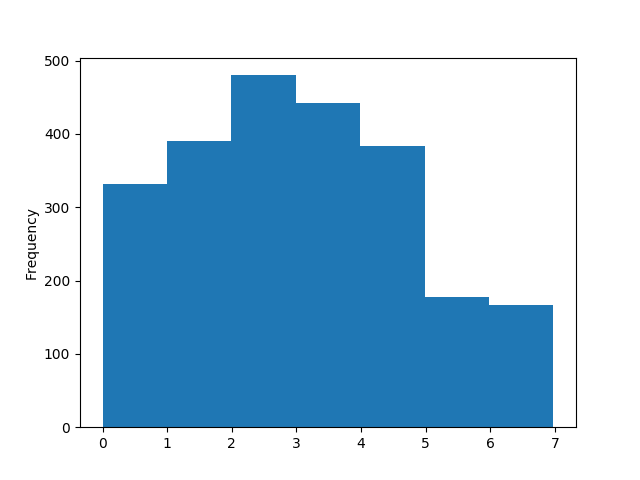
\includegraphics[width=\textwidth]{weekperiod_rough.png}
\end{frame}

\begin{frame}\frametitle{Commits over a Week}
\centering
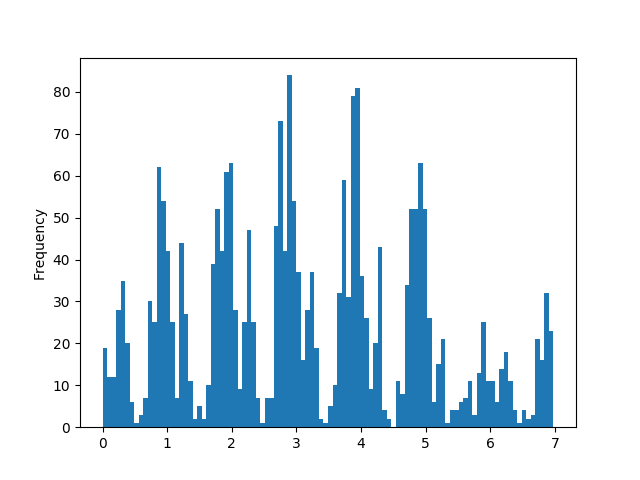
\includegraphics[width=\textwidth]{weekperiod.png}
\end{frame}

\begin{frame}\frametitle{Commits over a Day}
\centering
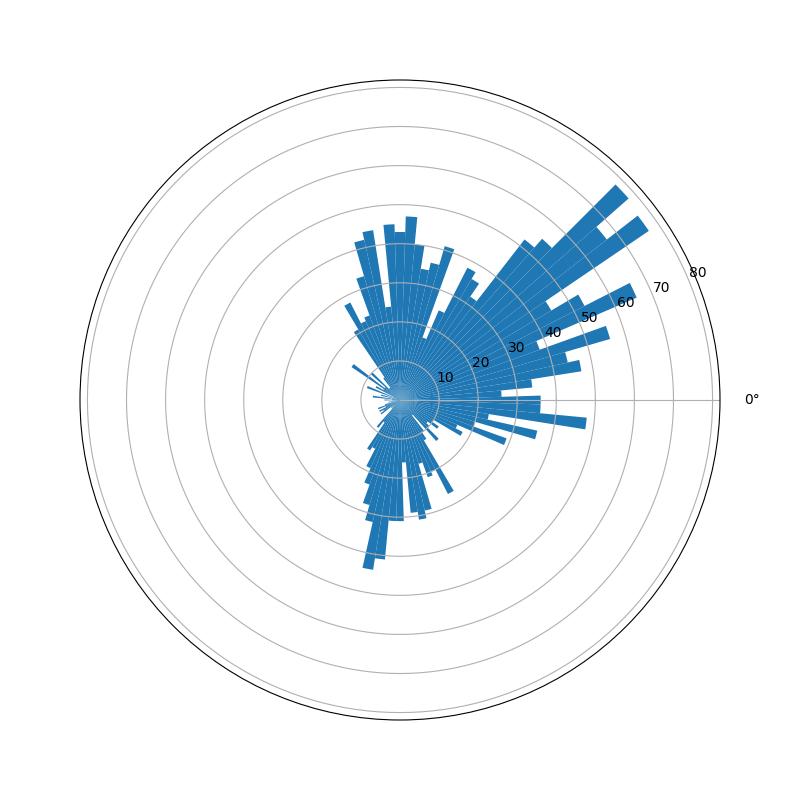
\includegraphics[width=0.8\textwidth]{dayperiod_polar.png}
\end{frame}

\begin{frame}\frametitle{Message Network}
\centering
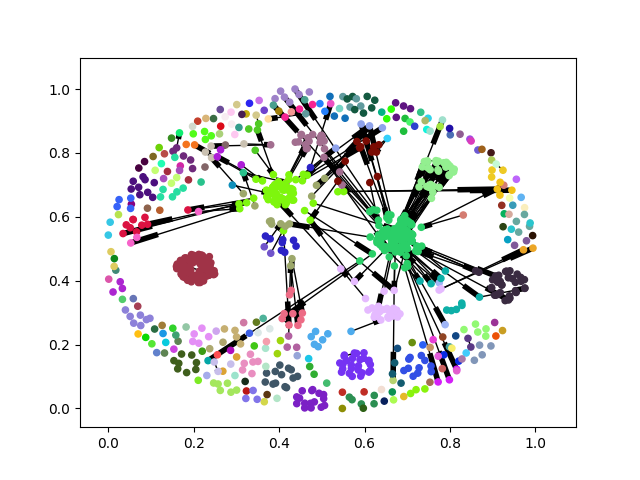
\includegraphics[width=1\textwidth]{messagegraph.png}
\end{frame}
\begin{frame}\frametitle{Boring People}
\centering
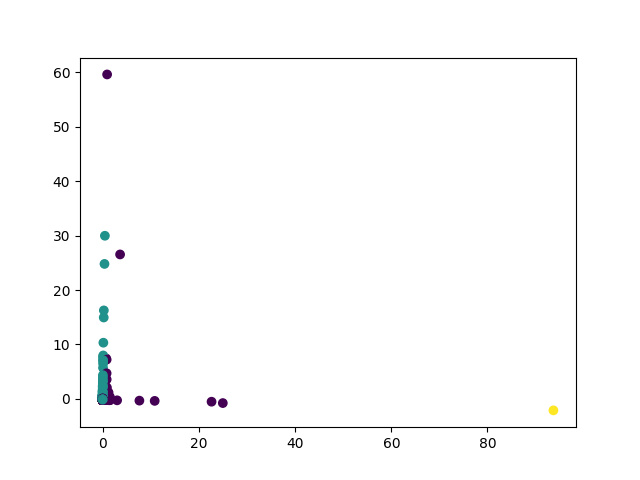
\includegraphics[width=1\textwidth]{cluster.png}
\end{frame}
\begin{frame}\frametitle{Boring People}
\centering
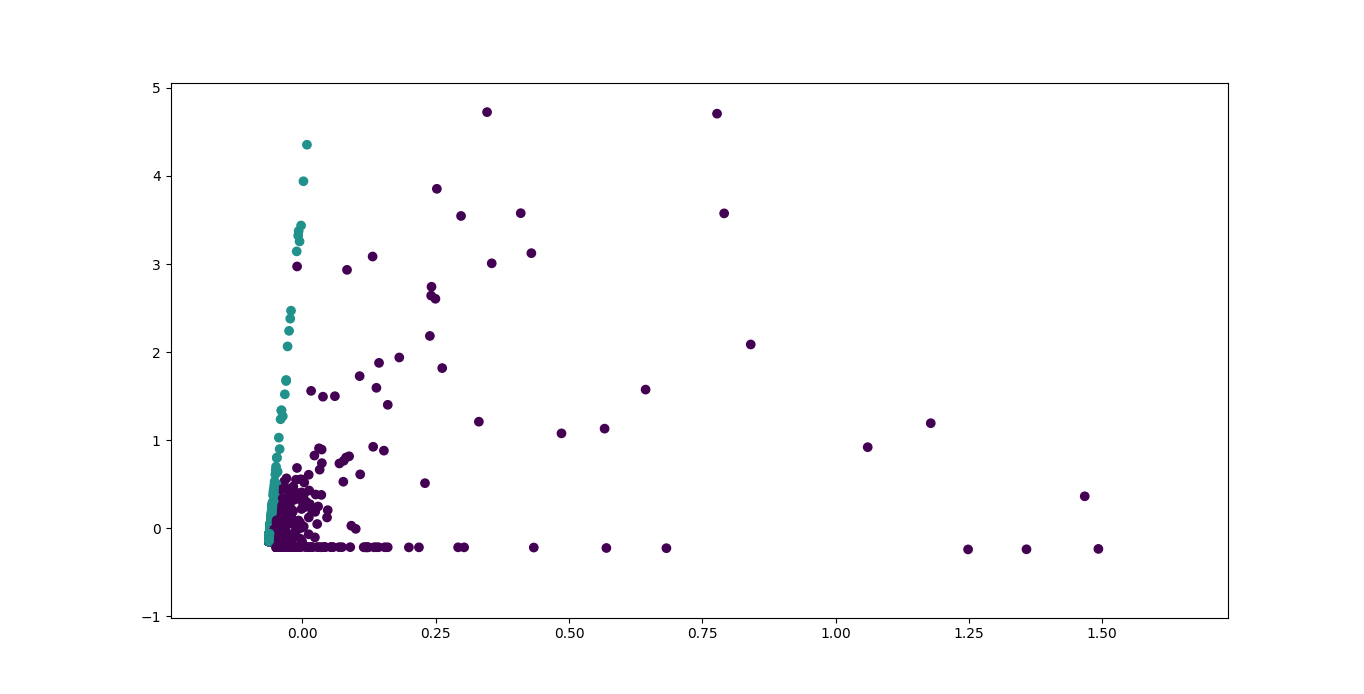
\includegraphics[width=1\textwidth]{cluster_zoom.png}
\end{frame}
\begin{frame}\frametitle{People Network}
\centering
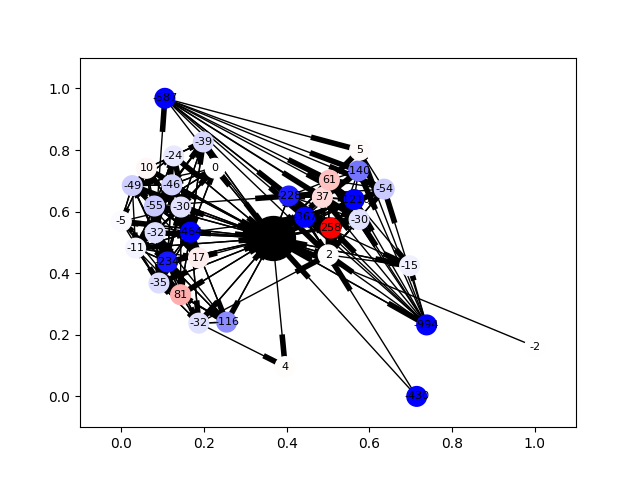
\includegraphics[width=\textwidth]{graph1.png}
\end{frame}
\begin{frame}\frametitle{People Network}
\centering
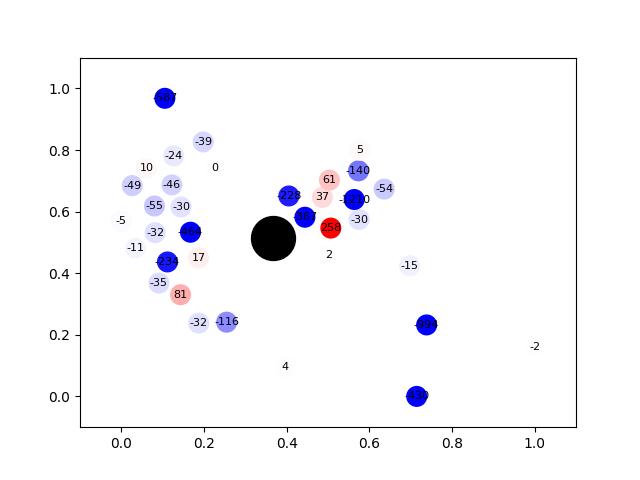
\includegraphics[width=\textwidth]{graph2.png}
\end{frame}
\begin{frame}\frametitle{People Network: Two Groups}
\centering
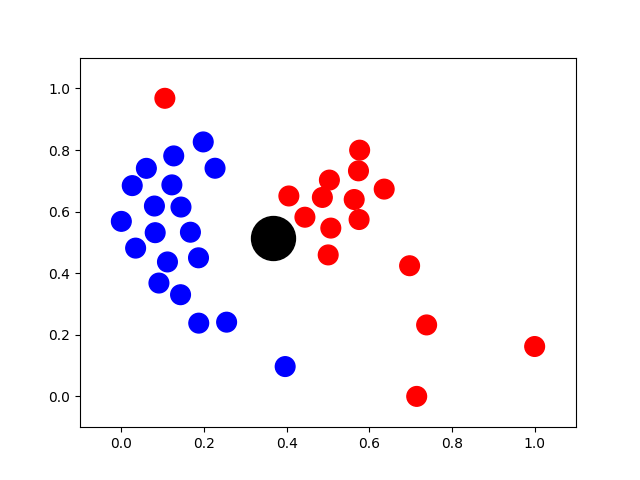
\includegraphics[width=\textwidth]{graph3.png}
\end{frame}
\begin{frame}\frametitle{People Network: JIRA}
\centering
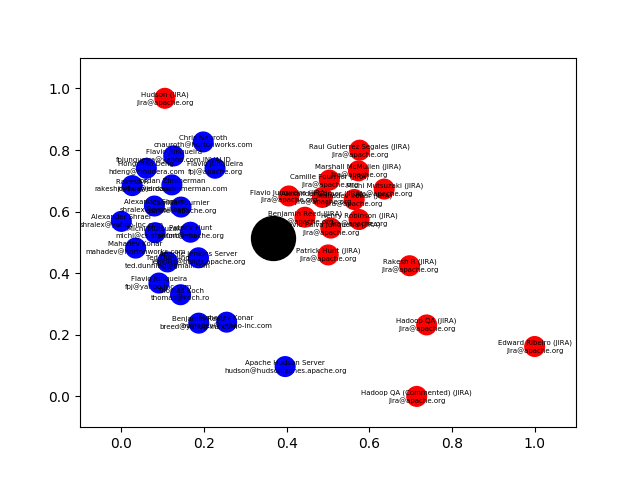
\includegraphics[width=\textwidth]{graph4.png}
\end{frame}
\begin{frame}\frametitle{People Network: JIRA}
\centering
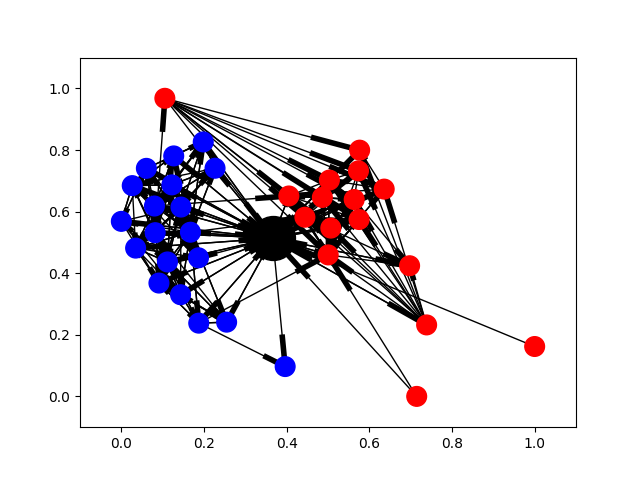
\includegraphics[width=\textwidth]{graph5.png}
\end{frame}
\begin{frame}\frametitle{People Network: Volume}
\centering
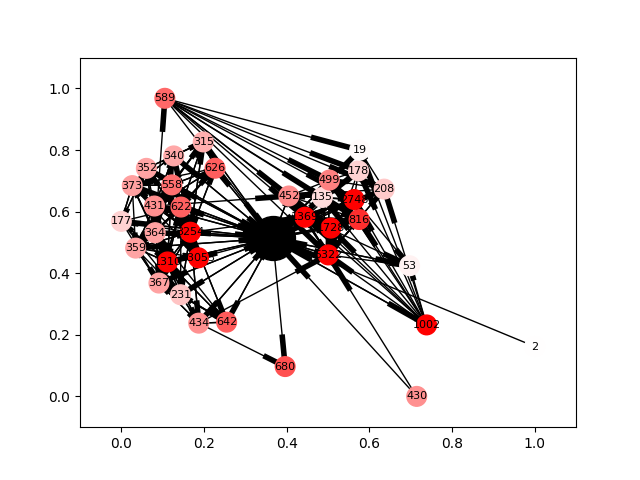
\includegraphics[width=\textwidth]{graph6.png}
\end{frame}
\begin{frame}\frametitle{People Network: Outvolume}
\centering
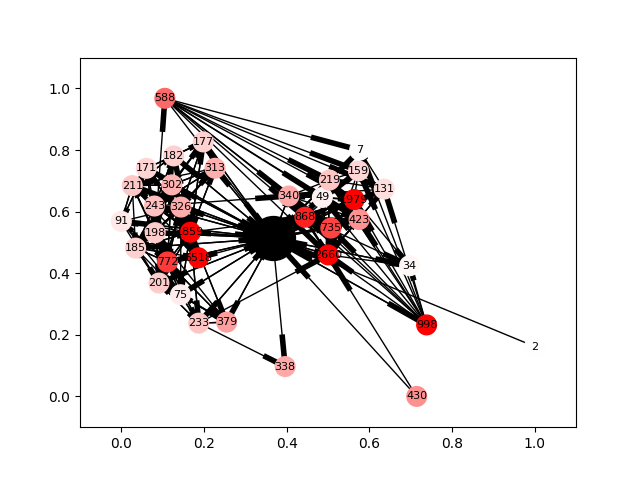
\includegraphics[width=\textwidth]{graph7.png}
\end{frame}
\begin{frame}\frametitle{People Network: Differential Volume}
\centering
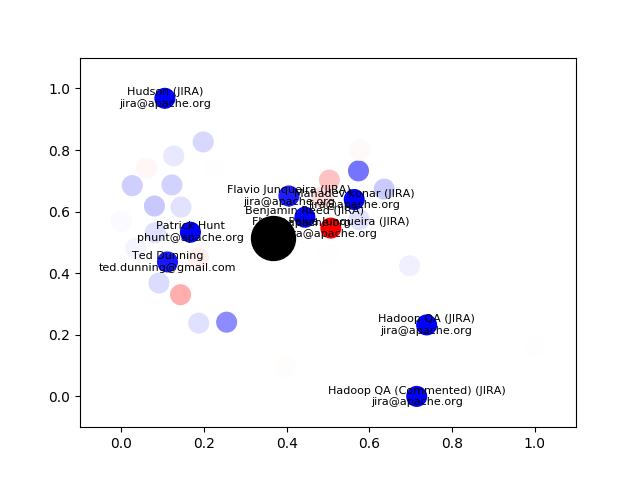
\includegraphics[width=\textwidth]{graph8.png}
\end{frame}

\begin{frame}\frametitle{Issue Priorities: Activity}
\centering
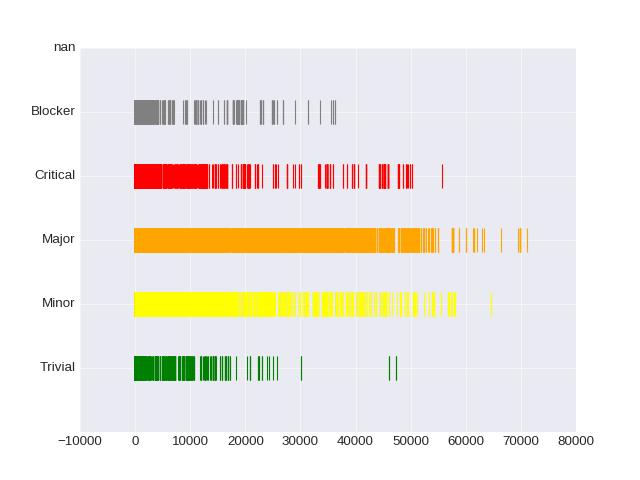
\includegraphics[width=\textwidth]{./issue_event_activity.png}
\end{frame}

\begin{frame}\frametitle{Issue Priorities: Resolvement}
\centering
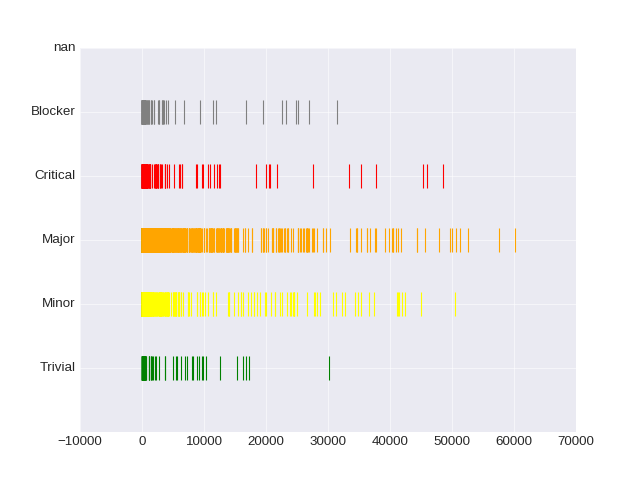
\includegraphics[width=\textwidth]{./issue_solve.png}
\end{frame}

\begin{frame}\frametitle{Issue Priorities: Medians}
\centering
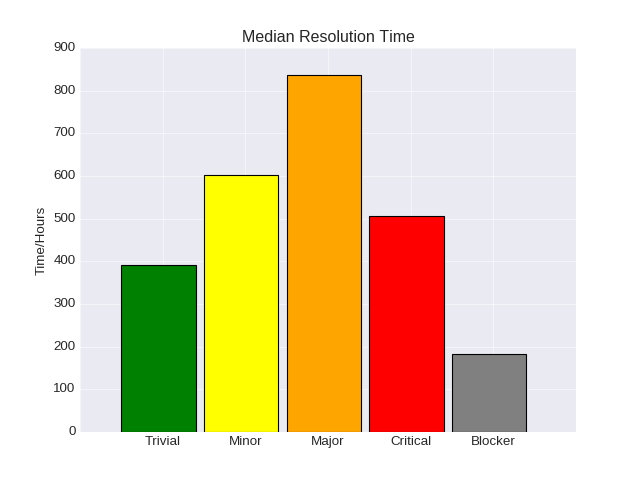
\includegraphics[width=\textwidth]{./median_resolution_time.png}
\end{frame}


\begin{frame}\frametitle{PCA}
\thispagestyle{empty}
\begin{figure}
\hspace{-3cm}
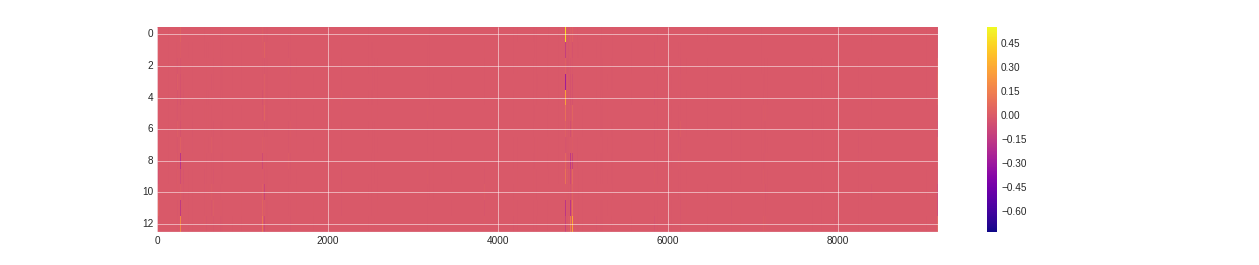
\includegraphics[width=1.5\textwidth]{./pca_components.png}
\end{figure}
\end{frame}


\begin{frame}\frametitle{Issue Clustering}
\centering
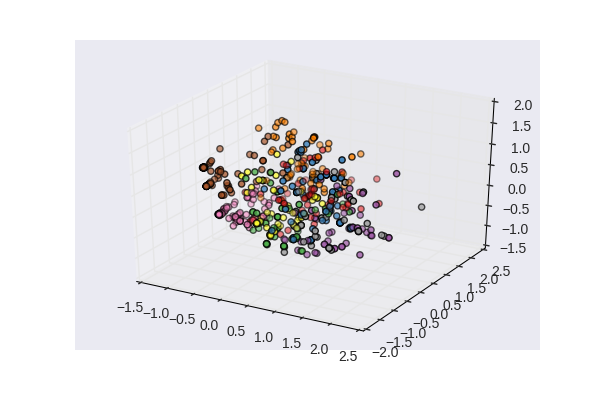
\includegraphics[width=\textwidth]{./clustering.png}
\end{frame}
\end{document}
